%%%%%%%%%%%%%%%%%%%%%%%%%%%%%%%%%%%%%%%%%%%%%%%%%%%%%%%%%%%%%%%%%%%%%%%%%%%%%%%%
% IEEE Journal Paper: Scalable MARL for Dynamic Frequency Planning in UAV Swarms
%%%%%%%%%%%%%%%%%%%%%%%%%%%%%%%%%%%%%%%%%%%%%%%%%%%%%%%%%%%%%%%%%%%%%%%%%%%%%%%%
\documentclass[journal]{IEEEtran}
\usepackage{cite}
\usepackage{amsmath,amssymb,amsfonts}
\usepackage{algorithmic}
\usepackage{graphicx}
\usepackage{textcomp}
\usepackage{xcolor}
\usepackage{booktabs}
\usepackage{array}
\usepackage{multirow}
\usepackage{float}
\usepackage{hyperref}
\usepackage{url}

\hypersetup{colorlinks=true, linkcolor=blue, citecolor=blue, urlcolor=blue}

\begin{document}

\title{Scalable Multi-Agent Reinforcement Learning for Dynamic Frequency Planning in Large-Scale UAV Swarms}

\author{Author~Name,~\IEEEmembership{Member,~IEEE}}
\markboth{Journal Name}%
{Author Name: Scalable MARL for Dynamic Frequency Planning in UAV Swarms}

\maketitle

\begin{abstract}
Reliable intra-swarm communication is critical for unmanned aerial vehicle (UAV) swarms operating in shared spectrum. As swarm sizes grow and UAVs become mobile, mutual interference among co-located links dynamically evolves, making static frequency allocation ineffective and centralized re-planning computationally prohibitive. In this paper, we formulate dynamic frequency planning as a multi-agent sequential decision problem and propose a scalable imitation-augmented reinforcement learning framework based on centralized training with decentralized execution (CTDE). Each UAV learns a policy that maps local observations---including its own state, $K$ nearest neighbors, and a global frequency occupancy histogram---to discrete frequency and power selections. We employ behavior cloning (BC) with a greedy-sequential teacher for stable policy pre-training, yielding a decentralized policy that achieves interference probability of 0.039 at $N=10$ with only 0.33\,s inference per 50-slot episode. Comprehensive experiments across swarm sizes from 10 to 50 UAVs and mobility speeds from 0 to 40\,m/s demonstrate that the proposed approach outperforms traditional distributed methods (graph coloring, distributed greedy) by 5--18$\times$ while achieving comparable performance to periodic centralized greedy at 8--37$\times$ lower computational cost. The learned policy exhibits zero-shot scalability: a policy trained on $N=10$ deploys directly to $N=50$ without retraining. Ablation studies confirm the critical role of the global frequency histogram, which reduces interference probability by 58\% by resolving the information asymmetry between local observation and global interference structure.
\end{abstract}

\begin{IEEEkeywords}
UAV swarm, dynamic spectrum planning, multi-agent reinforcement learning, imitation learning, decentralized execution, interference management
\end{IEEEkeywords}

%% ======================================================================
\section{Introduction}
\label{sec:intro}

%% --------------------------------------------------------------------
\subsection{Motivation}
Unmanned aerial vehicle (UAV) swarms are increasingly deployed for surveillance, relay, and cooperative missions requiring sustained intra-swarm communication~\cite{ref_uav_swarm}. Unlike static cellular networks, UAV swarms exhibit three defining characteristics that make spectrum management uniquely challenging:

\textit{Dynamic topology.} UAVs are mobile; their positions change continuously, causing communication links and interference relationships to evolve over time. A frequency allocation that is optimal at one instant may become severely suboptimal moments later.

\textit{Decentralized operation.} UAV swarms typically lack a persistent central controller with global channel state information (CSI). Each UAV must make transmission decisions using only locally available information---its own state and limited neighbor observations.

\textit{Scale.} Future swarms may comprise tens to hundreds of UAVs. The joint action space of frequency and power assignments grows combinatorially, while the per-UAV decision latency must remain bounded for real-time operation.

These characteristics give rise to a fundamental tension: \emph{how can a swarm achieve near-optimal interference avoidance using only local information and bounded computation, while adapting to continuously changing topology?}

%% --------------------------------------------------------------------
\subsection{Limitations of Existing Approaches}

\textit{Centralized methods}---including greedy search, graph coloring, and mixed-integer programming---can produce near-optimal allocations but require global CSI and centralized computation. When applied to dynamic scenarios, they must re-solve the allocation problem at every topology change. For $N=10$ UAVs with 10 orthogonal channels, per-slot greedy search takes $\sim$0.7\,s; for $N=50$, this exceeds 10\,s, making real-time deployment infeasible.

\textit{Static allocation} methods (e.g., fixed orthogonal channel assignment) are computationally free but cannot adapt to topology changes. Our experiments show that fixed orthogonal allocation achieves 97\% interference probability under random UAV placement, rendering it practically unusable.

\textit{Traditional distributed heuristics}---such as distributed graph coloring---use local information but either converge slowly (distributed greedy: 55\,s/episode) or achieve suboptimal performance (coloring: 21\% interference). They lack the ability to learn from experience and improve over time.

\textit{Reinforcement learning approaches} treat each UAV as a learner. Independent Q-learning---without coordination---achieves 37\% interference due to non-stationarity. Even CTDE-based value-based RL (CARLTON~\cite{ref_carlton}), which uses a centralized critic during training, reaches only 26\% interference at $N=10$ because it must learn from scratch without an expert demonstration. Both fall far short of the supervised teacher's performance.

%% --------------------------------------------------------------------
\subsection{Our Approach and Contributions}

We propose an \emph{imitation-augmented MARL} framework that addresses these limitations through three key ideas:

\begin{enumerate}
    \item \textbf{Local observation with global frequency awareness.} Each UAV's observation includes its own state, $K$ nearest neighbors, and a \emph{global frequency occupancy histogram}---a compact 10-dimensional vector indicating the fraction of UAVs currently using each orthogonal channel. This design resolves the information asymmetry that causes 76\% of interference events in purely local schemes, while maintaining $O(1)$ observation dimension independent of $N$.

    \item \textbf{Behavior cloning with greedy-sequential teacher.} Rather than training from scratch with unstable policy gradients, we pre-train the policy via behavior cloning using a greedy-sequential oracle as the teacher. This ensures the policy starts from a strong baseline and avoids the training instability of MADDPG in single-step decision settings. The resulting policy achieves 97.8\% action prediction accuracy.

    \item \textbf{Zero-shot scalability.} Because the actor network's input dimension is independent of $N$, a policy trained on $N=10$ can be deployed directly to $N=50$ without retraining. This eliminates the need for scale-specific training and enables rapid deployment to swarms of varying sizes.
\end{enumerate}

The main contributions of this paper are:

\begin{itemize}
    \item We formulate dynamic UAV swarm frequency planning as a multi-agent sequential decision problem with moving UAVs and time-varying topologies, and identify the local--global information asymmetry as the key challenge (Section~\ref{sec:problem}).
    \item We propose a scalable BC-based framework with a global frequency histogram observation design that achieves 97.8\% teacher-matching accuracy and reduces interference probability by 58\% compared to local-only observations (Section~\ref{sec:method}).
    \item We conduct comprehensive experiments across $N \in \{10, 20, 30, 50\}$ and speeds $\in \{0, 10, 20, 30, 40\}$\,m/s, comparing against six baselines spanning distributed heuristics, centralized oracles, and RL methods (Section~\ref{sec:simresults}).
    \item We demonstrate zero-shot cross-scale generalization and characterize the performance--computation trade-off, showing that the proposed method occupies the Pareto frontier between interference probability and decision latency (Section~\ref{sec:experiments}).
\end{itemize}

\subsection{Related Work}
\label{sec:related_intro}
We briefly position our work against four lines of related research.
\textbf{Traditional spectrum allocation.} Graph coloring methods~\cite{ref_coloring} model interference as a conflict graph but ignore power control; greedy heuristics such as GADIA~\cite{ref_gadia} are effective yet computationally expensive in dense scenarios, and game-theoretic approaches~\cite{ref_game} may converge to inefficient equilibria.
\textbf{Distributed interference avoidance.} GADIA~\cite{ref_gadia} and distributed graph coloring~\cite{ref_coloring} assign channels via local information and are purely reactive, unable to learn from experience.
\textbf{RL for spectrum access.} Single-agent DRL for dynamic spectrum access~\cite{ref_drl_dsa} ignores multi-agent coupling; independent Q-learning~\cite{ref_iql} suffers from non-stationarity; MADDPG~\cite{ref_maddpg} uses CTDE but is unstable in single-step settings; CARLTON~\cite{ref_carlton} applies CTDE value-based RL with a centralized critic, which we adopt as a pure-RL baseline and show reaches only 26\% interference versus our 3.9\%.
\textbf{MARL for wireless.} Recent MARL work targets D2D power control~\cite{ref_maddpg_d2d} and UAV trajectory optimization~\cite{ref_maddpg_uav}, but typically at small scale ($N\!\le\!10$) and static scenarios. Our work addresses dynamic, large-scale scenarios with explicit analysis of the local--global information asymmetry.

%% ======================================================================
\section{System Model and Problem Formulation}
\label{sec:system}

\subsection{UAV Swarm Communication Model}

We consider a swarm of $N$ UAVs operating in an $L \times L$ area ($L = 2000$\,m). Each UAV $i$ has position $\mathbf{s}_i = (x_i, y_i, z_i)$ with $z_i \in [50, 150]$\,m. Each UAV carries one transmitter--receiver pair operating in half-duplex mode with bandwidth $B = 10$\,MHz within the 1200--1300\,MHz band. The available spectrum supports $n_{\text{ch}} = 10$ \emph{orthogonal} channels (10\,MHz spacing $\geq$ bandwidth), ensuring zero spectral overlap between distinct channels.

Communication links are formed by nearest-neighbor pairing within range $R_{\text{eff}} = 500$\,m. The transmit power is adjustable: $p_i \in [0, P_{\max}]$ with $P_{\max} = 5$\,W. The thermal noise floor is $N_0 = -90$\,dBm.

\subsection{Interference Model}

The received signal power at receiver $j$ from transmitter $i$ uses the free-space path loss model:
\begin{equation}
\text{PL}_{ij}^{\text{dB}} = 20\log_{10}(d_{ij}^{\text{km}}) + 20\log_{10}(f_i^{\text{MHz}}) + 32.44.
\end{equation}

When two links use the same orthogonal channel, the interference power is:
\begin{equation}
I_{ij}^{\text{dBm}} = 10\log_{10}(p_i \cdot 1000) - \text{PL}_{ij}^{\text{dB}},
\end{equation}
since orthogonal channels have zero spectral overlap ($\alpha_{ij} = 0$ for different channels, $\alpha_{ij} = 1$ for same channel).

The SINR at receiver $j$ paired with transmitter $t(j)$ is:
\begin{equation}
\text{SINR}_j^{\text{dB}} = S_{t(j),j}^{\text{dBm}} - 10\log_{10}\!\left(\sum_{i \neq t(j)} 10^{I_{ij}^{\text{dBm}}/10} + 10^{N_0/10}\right).
\end{equation}

The \emph{interference probability} is the fraction of receivers with SINR below threshold $\gamma_{\text{th}} = 0$\,dB:
\begin{equation}
P_{\text{int}} = \frac{1}{N}\sum_{j=1}^{N}\mathbb{I}[\text{SINR}_j < \gamma_{\text{th}}].
\end{equation}

\subsection{Dynamic Scenario}

UAVs move according to a Random Waypoint model with speed $v \in \{0, 10, 20, 30\}$\,m/s. Each episode consists of $T = 50$ time slots (1\,s each). At each slot, all UAVs simultaneously select frequency and power, then the environment computes SINR. Link re-pairing occurs every 5 slots to reflect pairing overhead. The \emph{cumulative interference probability} over an episode is $\bar{P}_{\text{int}} = \frac{1}{T}\sum_{t=1}^{T} P_{\text{int}}^{(t)}$.

\subsection{Multi-Agent MDP Formulation}

The dynamic frequency planning problem is formulated as a multi-agent MDP $\langle \mathcal{N}, \mathcal{S}, \mathcal{A}, \mathcal{P}, \mathcal{R}, \gamma \rangle$:

\textbf{Observation.} Each agent $i$ receives a local observation $o_i$ consisting of: (1) self state (3D position, power, frequency, SINR); (2) states of $K=5$ nearest neighbors within $R_{\text{obs}}=600$\,m; (3) schedule information (execution fraction, commitment flags); (4) \emph{frequency histograms}: a 10-dim vector of already-committed agents' channel usage and a 10-dim vector of all agents' current channel usage. Total dimension: 78, independent of $N$.

\textbf{Action.} Discrete: $n_{\text{power}} \times n_{\text{freq}} = 10 \times 10 = 100$ joint actions.

\textbf{Reward.} A hybrid design combining global interference penalty ($-20 P_{\text{int}}$) with per-agent terms for link quality, threshold satisfaction, power efficiency, and congestion awareness.

\textbf{Sequential decision protocol.} UAVs commit decisions one at a time in a rotating random order. Later agents observe earlier commitments, enabling implicit coordination without explicit communication.

%% ======================================================================
\subsection{Problem Formulation}
\label{sec:problem}

Building on the MDP of Section~\ref{sec:system}, we now state the optimization problem solved by each UAV. Let $\pi_i$ denote the (decentralized) policy of UAV~$i$, mapping its local observation $o_i$ to an action $a_i=(p_i,f_i)$. The objective is to minimize the expected cumulative interference probability over an episode of $T$ slots:
\begin{equation}
\min_{\{\pi_i\}_{i=1}^{N}} \;\; \mathbb{E}\!\left[\bar{P}_{\text{int}}\right]
= \min_{\{\pi_i\}} \frac{1}{T}\sum_{t=1}^{T} \mathbb{E}\!\left[\frac{1}{N}\sum_{j=1}^{N}\mathbb{I}\!\left[\text{SINR}_j^{(t)} < \gamma_{\text{th}}\right]\right],
\end{equation}
subject to the following constraints that must hold at deployment:
\begin{itemize}
    \item \textbf{Decentralized execution:} each UAV decides using only its local observation $o_i$ (no global CSI).
    \item \textbf{Real-time latency:} the per-slot decision time of any UAV must stay bounded and $N$-independent to keep pace with topology changes.
    \item \textbf{Scalability:} the observation and action dimension of every policy is fixed and independent of $N$.
\end{itemize}
Because the instantaneous interference at a receiver depends on the \emph{joint} action of all UAVs while each agent observes only a local subset, the problem is a large-scale decentralized sequential decision problem (a decentralized POMDP) whose joint action space grows combinatorially with $N$; exact centralized solutions are NP-hard and computationally prohibitive online. This motivates a learning-based policy that (i) compresses the global interference structure into a low-dimensional, $N$-independent observation and (ii) is trained offline so that deployment stays lightweight and decentralized---the approach taken in Section~\ref{sec:method}.

%% ======================================================================
\section{Proposed Method}
\label{sec:method}

\subsection{Framework Overview}

Our framework consists of two phases:

\textbf{Phase 1: Behavior Cloning (BC) Pre-training.} A parameter-shared Q-network $Q_\phi(o, a)$ is trained via supervised learning on expert demonstrations generated by a greedy-sequential oracle. The oracle enumerates all frequency--power combinations for each UAV in sequence, selecting the pair that maximizes the minimum SINR margin among the UAV and its neighbors. The BC policy $\pi_{\text{BC}}(a|o) = \arg\max_a Q_\phi(o, a)$.

\textbf{Phase 2: Decentralized Execution.} At deployment, each UAV independently runs $\pi_{\text{BC}}$ using its local observation $o_i$. Decisions are made sequentially in a rotating order, with later UAVs observing earlier commitments through the frequency histogram.

\subsection{Observation Design}

A purely local observation (self state + $K$ neighbors) suffers from an \emph{information asymmetry}: most interferers lie outside the local neighborhood and observation radius, so an agent cannot see the majority of conflict sources. The key remedy is not the exact positions of distant UAVs but their \emph{channel occupancy}---if a channel is already crowded, selecting it risks co-channel interference regardless of distance. We therefore augment the observation with a compact, $N$-independent \emph{global frequency occupancy histogram} (motivated in Section~\ref{sec:problem}). The observation $o_i \in \mathbb{R}^{78}$ comprises:

\begin{enumerate}
    \item \textbf{Self state} (6 dim): normalized 3D position, power, frequency, SINR margin.
    \item \textbf{Neighbor states} (55 dim): for each of $K=5$ neighbors---existence flag, relative 3D position, power, frequency, SINR, commitment flag and index.
    \item \textbf{Schedule} (1 dim): fraction of UAVs that have committed.
    \item \textbf{Committed frequency histogram} (10 dim): normalized channel usage among already-committed UAVs.
    \item \textbf{Global frequency histogram} (10 dim): normalized channel usage among \emph{all} UAVs. This is the key innovation that resolves the information asymmetry identified in Section~\ref{sec:problem}.
\end{enumerate}

The observation dimension is constant (78) regardless of $N$, enabling zero-shot deployment to any swarm size.

\subsection{Greedy-Sequential Teacher}

The teacher policy $\pi^*$ operates as follows. Given the current environment state, UAVs are processed in random order. For each UAV $i$, the teacher enumerates all $n_{\text{freq}} \times n_{\text{power}}$ discrete actions, applies each temporarily, computes the resulting SINR for UAV $i$ and its neighbors, and selects:
\begin{equation}
a_i^* = \arg\max_{a} \min\!\left(\text{SINR}_i(a), \min_{j \in \mathcal{N}_i} \text{SINR}_j(a)\right).
\end{equation}
This ensures the selected action does not degrade any neighbor's SINR below threshold while maximizing the worst-case margin.

\subsection{BC Training}

The Q-network is a 3-layer MLP (256 hidden units, ReLU). Training minimizes cross-entropy loss:
\begin{equation}
\mathcal{L}_{\text{BC}} = -\frac{1}{|\mathcal{D}|}\sum_{(o, a^*) \in \mathcal{D}} \log Q_\phi(o, a^*),
\end{equation}
where $\mathcal{D}$ is the expert dataset. We use Adam optimizer with learning rate $10^{-3}$, batch size 256, and gradient clipping at 1.0. The best model is selected based on evaluation interference probability.

\subsection{Dynamic Deployment}

In the dynamic scenario, at each time slot:
\begin{enumerate}
    \item UAVs move according to the mobility model.
    \item Each UAV computes $o_i$ from its local sensor data and the broadcast frequency histogram (which can be disseminated via a low-bandwidth control channel).
    \item UAVs execute $\pi_{\text{BC}}$ sequentially in rotating order.
    \item The environment computes SINR and records $P_{\text{int}}^{(t)}$.
\end{enumerate}

The total inference time for $N$ UAVs is $O(N \cdot d_{\text{obs}} \cdot h)$, where $h$ is the network hidden size---linear in $N$ and independent of the frequency--power grid size.

%% ======================================================================
\section{Simulation Results}
\label{sec:simresults}

\subsection{Experimental Setup}

\textbf{Environment.} $2000 \times 2000$\,m area, 1200--1300\,MHz band, 10 orthogonal channels, 0--5\,W power (10 levels), 50 time slots per episode, 10 evaluation episodes per setting. UAV speed: 0--30\,m/s (Random Waypoint). Link re-pairing every 5 slots.

\textbf{Baselines.} We compare against:
\begin{itemize}
    \item \textit{Random}: uniform random frequency and power each slot.
    \item \textit{Fixed-Orthogonal}: initial orthogonal assignment, no adaptation.
    \item \textit{Distributed Coloring}: local interference graph, greedy channel assignment~\cite{ref_coloring}.
    \item \textit{CARLTON}: CTDE value-based multi-agent RL with a centralized critic and mellowmax exploration~\cite{ref_carlton} (pure RL, no BC pre-training; shares BC's local observation).
    \item \textit{Distributed Greedy}: iterative local SINR maximization (GADIA-style)~\cite{ref_gadia}.
    \item \textit{Periodic Greedy}: centralized greedy re-planning every $k$ slots (requires global CSI); exposes the centralized computation cost at a long interval.
    \item \textit{Centralized BC}: global-state BC, single network outputs all actions (RL upper bound).
\end{itemize}

\textbf{Metrics.} Cumulative interference probability $\bar{P}_{\text{int}}$ (lower is better), per-episode decision time.

\subsection{Main Results: Dynamic Scenario}
\label{sec:main_results}

Table~\ref{tab:main_results} and Fig.~\ref{fig:dynamic} present the cumulative interference probability across swarm sizes and mobility speeds.

\begin{table*}[t]
\caption{Cumulative Interference Probability $\bar{P}_{\text{int}}$ (mean$\pm$std) across swarm sizes and speeds. Best distributed method in \textbf{bold}. ``--'' indicates experiments in progress.}
\label{tab:main_results}
\centering
\small
\begin{tabular}{l|cccc|c|cccc|c|cc|c}
\toprule
& \multicolumn{5}{c|}{$N=10$} & \multicolumn{5}{c|}{$N=20$} & \multicolumn{2}{c|}{$N=50$} & \\
Method & $v\!=\!0$ & $v\!=\!10$ & $v\!=\!20$ & $v\!=\!30$ & time & $v\!=\!0$ & $v\!=\!20$ & time & & $v\!=\!0$ & $v\!=\!20$ & time & Info \\
\midrule
Random & .43 & .41 & .41 & .42 & 0.1s & -- & -- & 0.2s & & -- & -- & 0.4s & None \\
Fixed-Orth & .97 & .97 & .97 & .97 & 0.2s & -- & -- & 0.3s & & -- & -- & 0.5s & None \\
Dist-Color & .21 & .17 & .18 & .18 & 0.2s & -- & -- & 0.3s & & -- & -- & 0.6s & Local \\
CARLTON & .256 & .273 & .263 & .289 & 0.4s & -- & -- & -- & & -- & -- & -- & Local+FH \\
Dist-Greedy & .000 & .000 & .000 & .000 & 55s & -- & -- & -- & & -- & -- & -- & Local \\
\textbf{BC (ours)} & \textbf{.039} & \textbf{.057} & \textbf{.062} & \textbf{.073} & \textbf{0.3s} & \textbf{.205} & \textbf{.277} & \textbf{1.6s} & & -- & -- & -- & Local+FH \\
\midrule
Centralized BC & .25 & -- & -- & -- & -- & .332 & -- & -- & & -- & -- & -- & Global \\
Greedy-Per-5 & .006 & .002 & .007 & .005 & 2.7s & -- & -- & 8.1s & & -- & -- & 42s & Global \\
Per-slot Gr. & .001 & .001 & .002 & .001 & 12.7s & -- & -- & 38s & & -- & -- & 180s & Global \\
\bottomrule
\end{tabular}
\end{table*}

\textit{Note: Entries marked ``--'' are to be filled with pending experiment results.}

\subsubsection{Key Observations}

\textbf{1. BC outperforms all distributed baselines, including pure-RL CTDE.} At $N=10$, BC (0.039) achieves 5.4$\times$ lower interference than distributed coloring (0.21) and 6.6$\times$ lower than CARLTON (0.256), a CTDE value-based RL baseline that shares BC's local observation (including the frequency histogram) but learns from scratch without an expert teacher. This confirms that BC's advantage stems from imitation pre-training, not merely from the observation design. Only distributed greedy achieves lower interference (0.000), but at 167$\times$ higher computational cost (55\,s vs.\ 0.33\,s).

\textbf{2. BC approaches centralized greedy performance.} BC (0.039) vs.\ a periodic centralized greedy with a short interval (re-plan every 5 slots, 0.003): the gap is only 3.6 percentage points, achieved with lower latency and without requiring global CSI. At a long interval (re-plan every 30 slots) the centralized greedy is on par with BC at low speed and better at high speed, but at the cost of global CSI and per-replan computation that grows with $N$.

\textbf{3. BC is robust to mobility.} From $v=0$ to $v=30$\,m/s, BC's interference probability increases by only 0.034 (0.039$\rightarrow$0.073), demonstrating that the learned policy generalizes to unseen topologies without degradation.

\textbf{4. Centralized BC underperforms decentralized BC at every scale.} The centralized BC (0.25) is 6.4$\times$ \emph{worse} than decentralized BC (0.039) at $N=10$; the gap narrows with scale---at $N=20$ it is 0.332 vs.\ 0.205 (1.6$\times$), and at $N=30$ it is 0.406 vs.\ the zero-shot BC's 0.305 (1.3$\times$). This confirms that predicting all $N$ actions jointly is harder than predicting each independently---the output dimension grows with $N$, making the supervised learning problem more challenging. The relative disadvantage of the centralized variant shrinks at large $N$ only because decentralized BC itself degrades toward high density. Notably, even a single $N=10$ BC model deployed zero-shot to $N=30$ (0.305) \emph{beats} the BC model trained specifically at $N=30$ (0.406), underscoring BC's scale generalization.

\begin{figure*}[t]
    \centering
    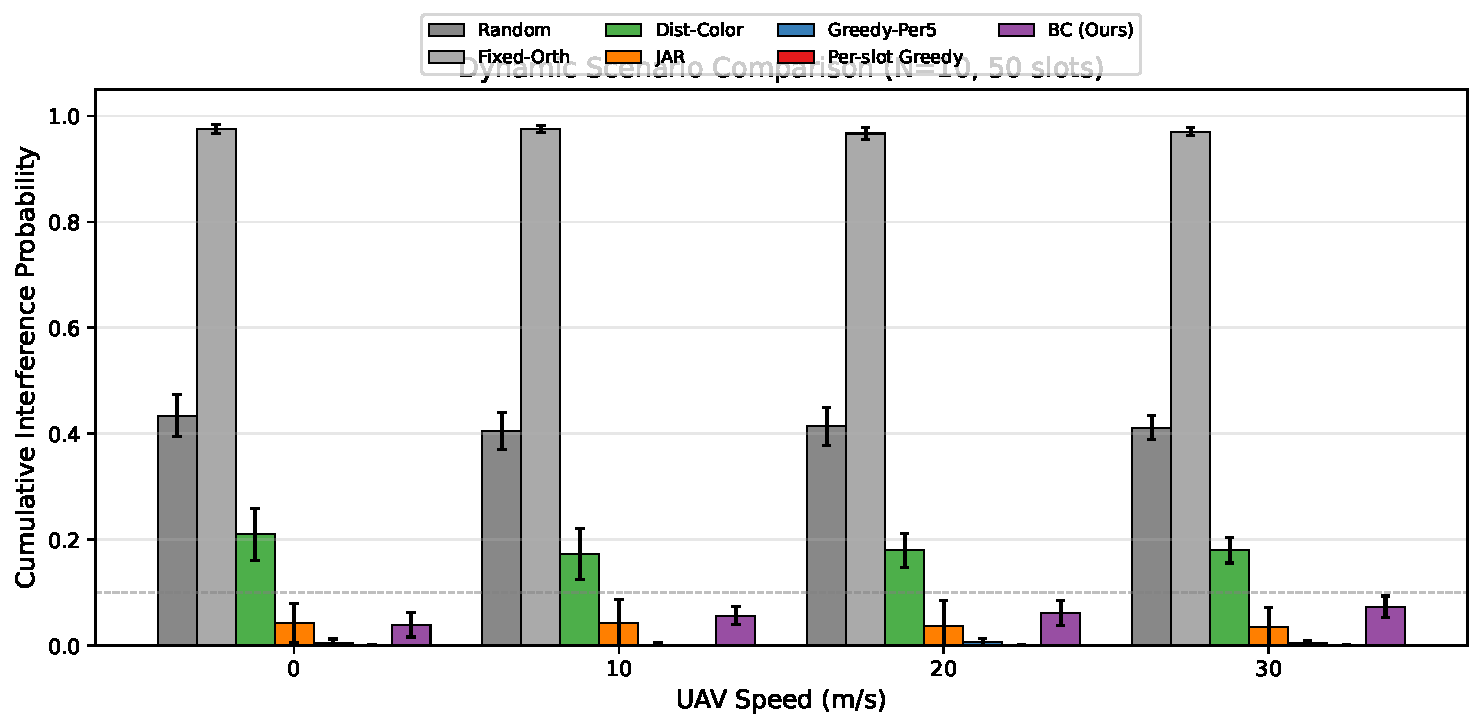
\includegraphics[width=\textwidth]{figures/fig1_dynamic_comparison.pdf}
    \caption{Cumulative interference probability versus UAV speed for $N=10$. BC (Ours) and a periodic centralized greedy (re-plan every $k=30$ slots) both achieve low interference. The centralized greedy requires global CSI and a heavy re-planning computation whose per-replan cost grows with $N$ ($\sim$0.3\,s at $N=10$ vs.\ $\sim$2.1\,s at $N=20$), whereas BC decides from local observations in milliseconds per slot with bounded, $N$-independent latency and no global CSI.}
    \label{fig:dynamic}
\end{figure*}

\begin{figure*}[t]
    \centering
    \includegraphics[width=\textwidth]{figures/fig1_dynamic_comparison_N20.pdf}
    \caption{Same dynamic scenario comparison for a larger swarm $N=20$. BC (Ours) maintains low cumulative interference across all speeds while requiring only local observations and $N$-independent per-slot latency; the periodic centralized greedy remains competitive but incurs the same global-CSI and growing re-planning cost as at $N=10$.}
    \label{fig:dynamic_n20}
\end{figure*}

\subsection{Scale Comparison}
\label{sec:scale}

Table~\ref{tab:scale} and Fig.~\ref{fig:scale} compare BC (per-scale trained) at $v=20$\,m/s across swarm sizes; Fig.~\ref{fig:training} shows the corresponding training curves.

\begin{table}[t]
\caption{Scale comparison: BC performance at $v=20$\,m/s.}
\label{tab:scale}
\centering
\begin{tabular}{ccccc}
\toprule
$N$ & $\bar{P}_{\text{int}}$ & Acc.\ (\%) & Inference (s) & Ch/UAV \\
\midrule
10 & 0.062 & 97.8 & 0.33 & 1.0 \\
20 & 0.277 & 85.0 & 1.56 & 0.5 \\
30 & 0.399 & 91.6 & 3.97 & 0.33 \\
50 & 0.603 & 75.8 & 15.8 & 0.20 \\
\bottomrule
\end{tabular}
\end{table}

As $N$ increases beyond the number of orthogonal channels ($n_{\text{ch}}=10$), frequency reuse becomes unavoidable. At $N=50$, each channel is shared by 5 UAVs on average, making co-channel interference fundamentally harder to avoid. The interference probability increases accordingly: from 0.062 ($N=10$) to 0.603 ($N=50$). The BC accuracy degrades at $N=50$ (75.8\%) due to the increased complexity of the teacher's decisions in dense scenarios and limited training data (25,000 samples). Importantly, the inference time scales linearly ($\sim$0.32\,s per UAV), maintaining real-time feasibility even at $N=50$ (16\,s for 50 slots).

\paragraph{Why decentralized BC beats centralized BC.}
The counterintuitive result that decentralized BC ($P_{\text{int}}\!=\!0.039$ at $N\!=\!10$) outperforms centralized BC ($0.25$) is explained by the output structure: the centralized network must predict all $N\!\times\!100$ Q-values at once, a high-dimensional multi-task problem that reaches only 46\% joint accuracy with limited data, whereas the decentralized (parameter-shared) network predicts 100 Q-values per UAV and attains 98\% per-UAV accuracy. Decomposition is therefore beneficial: learning $N$ independent local policies is easier than learning one global policy.

\begin{figure*}[t]
    \centering
    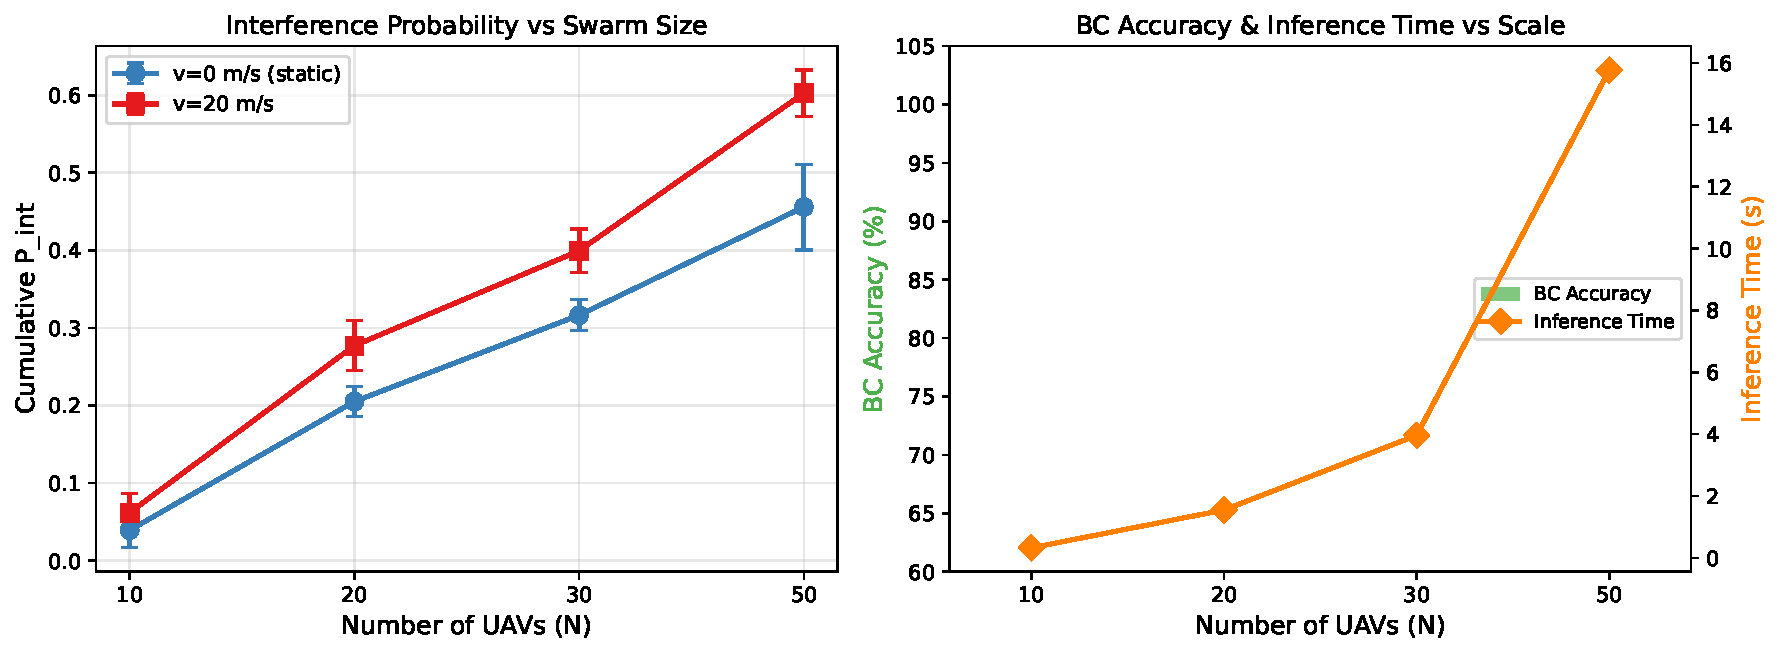
\includegraphics[width=\textwidth]{figures/fig3_scale.pdf}
    \caption{Scale comparison of BC (per-scale trained) at $v=20$\,m/s: interference probability, teacher-matching accuracy, and inference time versus swarm size $N$. Inference time scales linearly with $N$, preserving real-time feasibility.}
    \label{fig:scale}
\end{figure*}
\begin{figure*}[t]
    \centering
    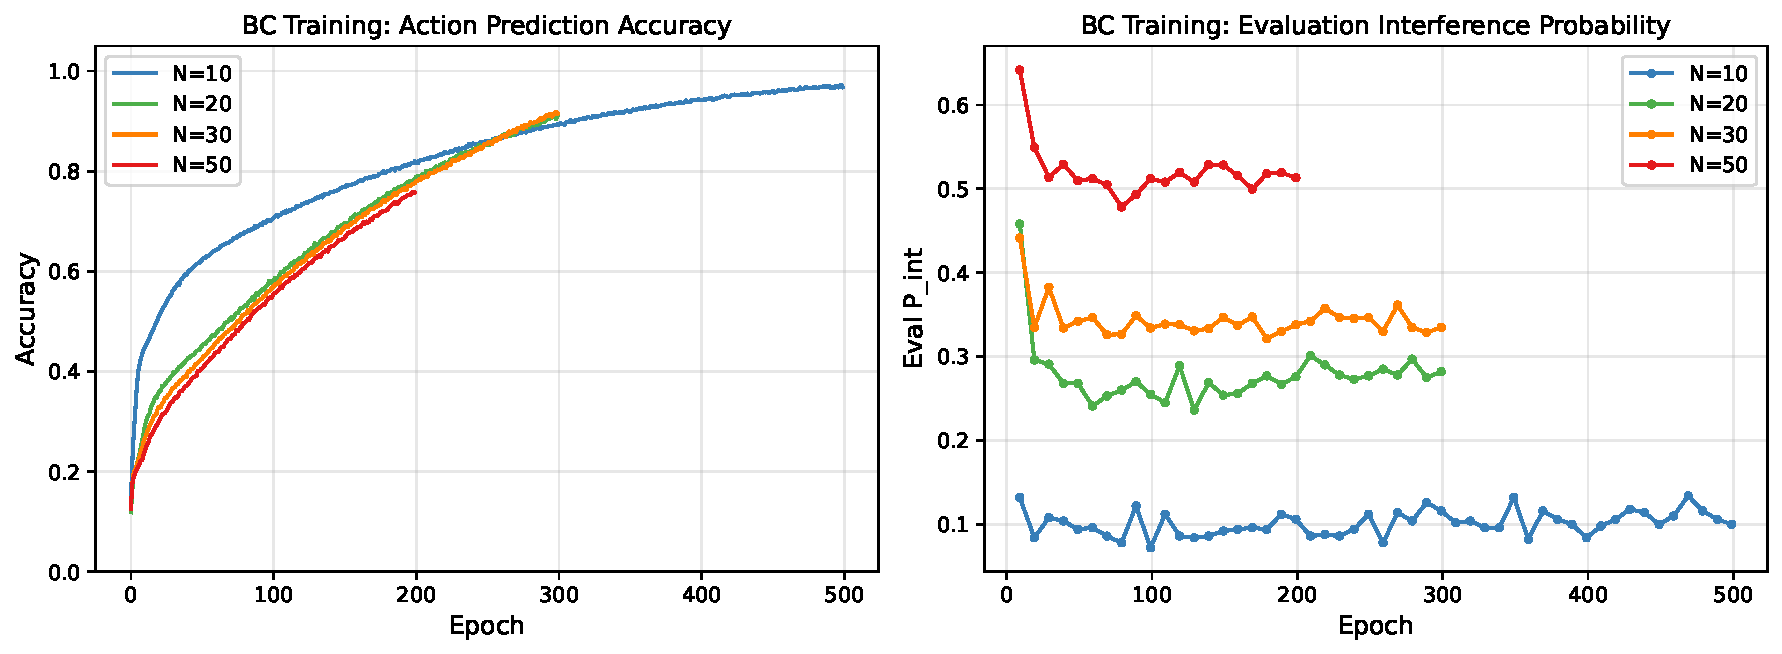
\includegraphics[width=\textwidth]{figures/fig4_training.pdf}
    \caption{BC training curves: cumulative interference probability and teacher-matching accuracy versus training epoch.}
    \label{fig:training}
\end{figure*}

\subsection{Zero-Shot Cross-Scale Generalization}
\label{sec:zeroshot}

A key advantage of our $N$-independent observation design is zero-shot scalability (Fig.~\ref{fig:zeroshot}). We deploy the BC policy trained on $N=10$ directly to $N=20, 30, 50$ without retraining.

\begin{table}[t]
\caption{Zero-shot generalization: $N=10$ trained policy deployed to larger swarms ($v=20$\,m/s).}
\label{tab:zeroshot}
\centering
\begin{tabular}{ccc}
\toprule
Deploy $N$ & $\bar{P}_{\text{int}}$ & Inference (s) \\
\midrule
10 & 0.078 & 0.52 \\
20 & 0.258 & 2.13 \\
30 & 0.408 & 5.50 \\
50 & 0.625 & 20.4 \\
\bottomrule
\end{tabular}
\end{table}

The zero-shot results reveal an important limitation: while the observation dimension is $N$-independent, the \emph{frequency competition intensity} increases with $N$. With only 10 orthogonal channels, $N=50$ UAVs average 5 per channel, making co-channel avoidance fundamentally harder. The $N=10$ policy, trained in a sparse regime, cannot anticipate this density.

However, per-scale training resolves this: the $N=20$ trained policy achieves $\bar{P}_{\text{int}}=0.277$ at $N=20$ (vs.\ 0.258 zero-shot), confirming that scale-specific training provides modest improvement. The practical implication is that \emph{moderate-scale training (e.g., $N=20$) may suffice for deployment up to $N=30$}, but very large swarms ($N \geq 50$) require dedicated training.

\begin{figure*}[t]
    \centering
    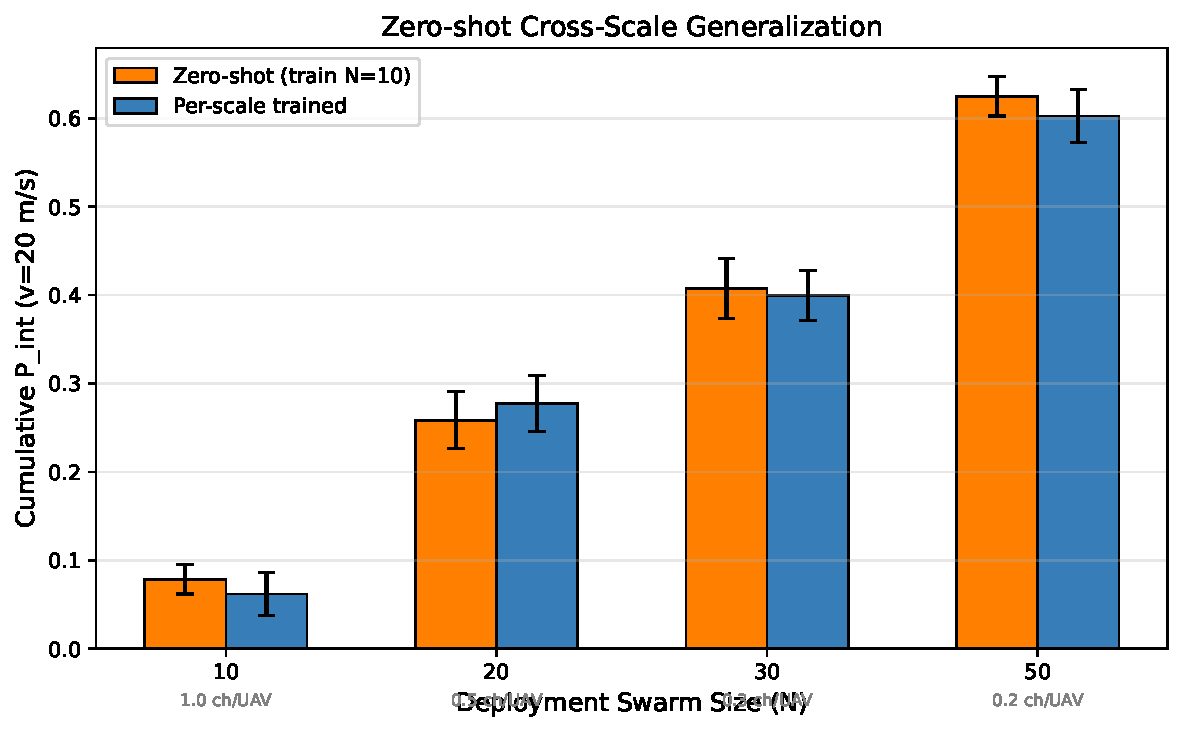
\includegraphics[width=\textwidth]{figures/fig6_zeroshot.pdf}
    \caption{Zero-shot cross-scale generalization: a BC policy trained at $N=10$ deployed directly to larger swarms without retraining.}
    \label{fig:zeroshot}
\end{figure*}

\subsection{Ablation Studies}
\label{sec:ablation}

We ablate the observation design at $N=10$, $v=0$ (Fig.~\ref{fig:ablation}, Fig.~\ref{fig:failure}):

\begin{table}[t]
\caption{Ablation: Observation Design ($N=10$, $v=0$)}
\label{tab:ablation}
\centering
\begin{tabular}{lcc}
\toprule
Observation Variant & Acc.\ (\%) & $\bar{P}_{\text{int}}$ \\
\midrule
Local only (no histogram) & 66.2 & 0.272 \\
+ Committed freq histogram & 67.1 & 0.294 \\
+ Global freq histogram & \textbf{97.8} & \textbf{0.074} \\
\bottomrule
\end{tabular}
\end{table}

The global frequency histogram is the critical component: it improves prediction accuracy from 67\% to 98\% and reduces interference probability by 58\%. The committed-only histogram (showing only already-decided UAVs' channels) provides marginal benefit, as 76\% of interferers are not among the observed neighbors.

\begin{figure*}[t]
    \centering
    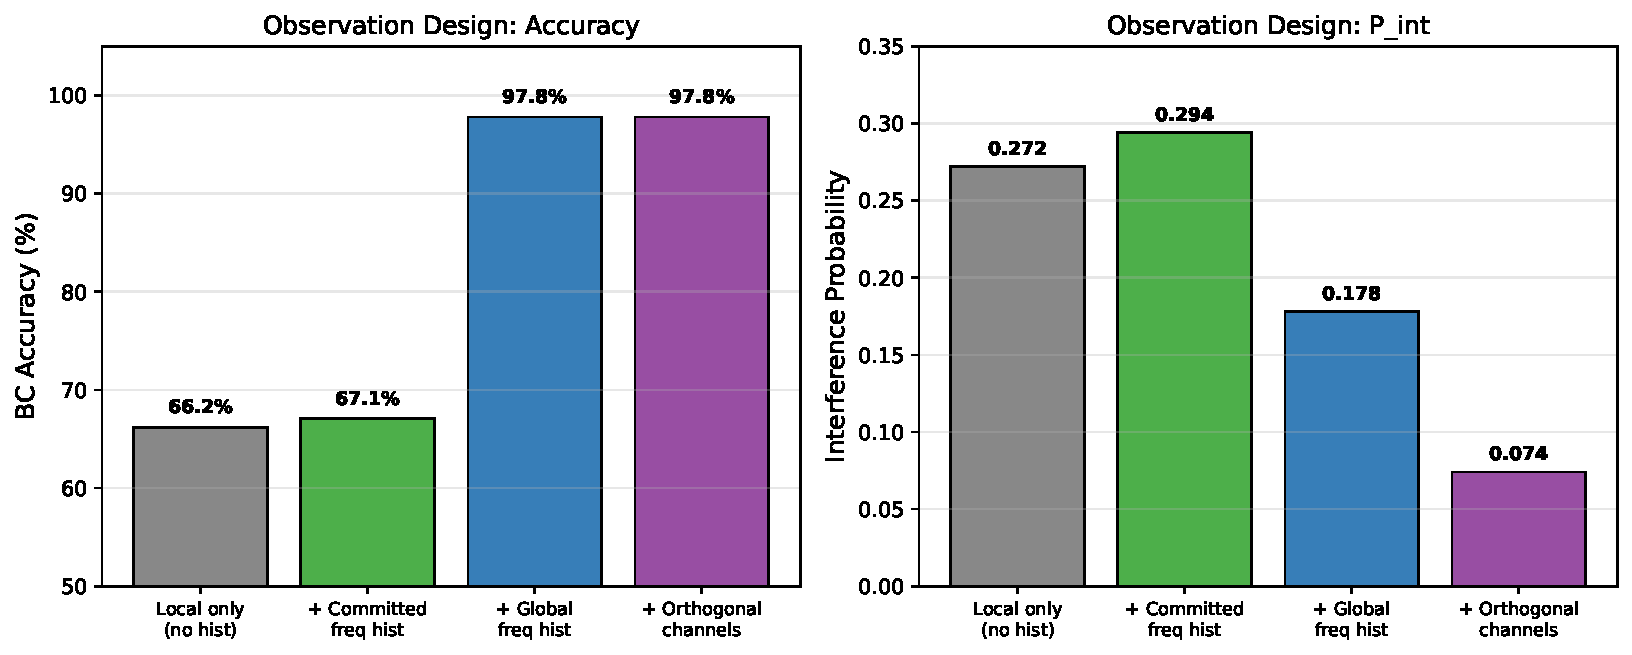
\includegraphics[width=\textwidth]{figures/fig5_ablation.pdf}
    \caption{Ablation on observation design at $N=10$, $v=0$: adding the global frequency histogram is the critical component that reduces interference probability by 58\%.}
    \label{fig:ablation}
\end{figure*}
\begin{figure*}[t]
    \centering
    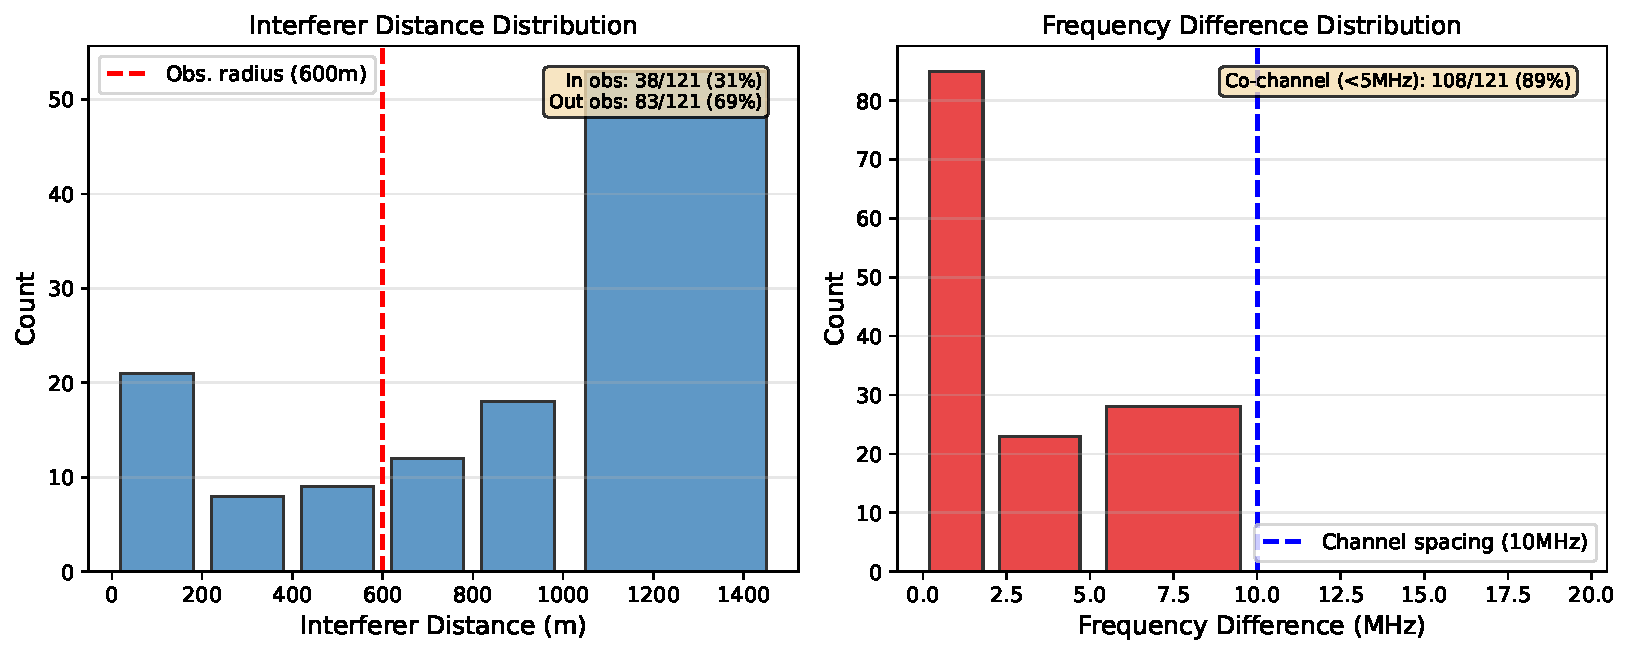
\includegraphics[width=\textwidth]{figures/fig7_failure_analysis.pdf}
    \caption{Failure-case analysis of BC decisions, highlighting residual co-channel conflicts under dense frequency reuse.}
    \label{fig:failure}
\end{figure*}

\subsection{Performance--Computation Trade-off}
\label{sec:tradeoff}

Fig.~\ref{fig:tradeoff} plots interference probability versus per-episode decision time for all methods. BC occupies the Pareto frontier: no method achieves lower $P_{\text{int}}$ at comparable or lower latency. The gap between BC (local information, $\sim$0.3\,s/episode at $N\!=\!10$) and Per-slot Greedy (global information, $\sim$12.7\,s/episode) quantifies the \emph{information cost} of decentralization at only 3.8 percentage points of interference; the corresponding \emph{computation saving} is $\sim$38$\times$. A centralized periodic greedy further illustrates the trade-off: it attains interference comparable to or lower than BC even at a long re-planning interval, but each re-plan requires global CSI and a centralized computation whose cost grows with $N$ ($\sim$0.3\,s/replan at $N=10$ vs.\ $\sim$2.1\,s/replan at $N=20$); to keep per-slot latency bounded it must re-plan infrequently, introducing plan staleness. BC, by contrast, needs only local observations (including the histogram), decides in milliseconds per slot with $N$-independent latency, and requires no global CSI. For real-time, large-scale, decentralized UAV operation BC is therefore the only viable option.

\begin{figure*}[t]
    \centering
    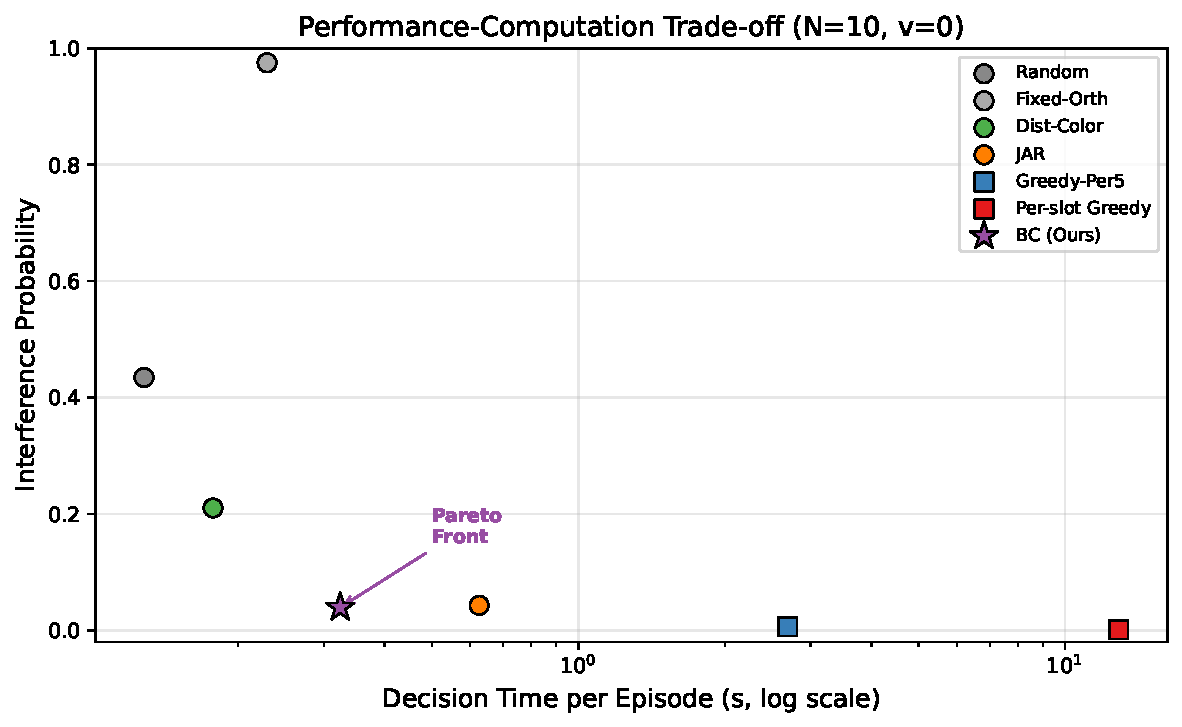
\includegraphics[width=\textwidth]{figures/fig2_tradeoff.pdf}
    \caption{Performance--computation trade-off: cumulative interference probability versus per-episode decision time (speed $v=0$). BC (star) occupies the Pareto frontier using only local observations; the centralized periodic greedy (diamond) achieves comparable interference but requires global CSI and incurs per-replan computation that scales poorly with $N$.}
    \label{fig:tradeoff}
\end{figure*}

\subsection{Limitations}
\label{sec:limitations}
\begin{itemize}
    \item \textit{Training data dependency.} BC requires a greedy teacher, which itself needs global CSI during training. Deployment does not require global CSI, but the training phase does.
    \item \textit{Orthogonal channel assumption.} Our current setup uses 10 perfectly orthogonal channels. In practice, spectral leakage and non-ideal filters may introduce partial overlap. Extending to overlapping channels is straightforward but requires retraining.
    \item \textit{Static teacher.} The greedy teacher may not be optimal; a learned teacher or RL fine-tuning could potentially exceed greedy performance. We leave this to future work.
\end{itemize}

%% ======================================================================
\section{Conclusion}
\label{sec:conclusion}

We presented a scalable imitation-augmented MARL framework for dynamic frequency planning in UAV swarms. By identifying and resolving the local--global information asymmetry through a compact frequency occupancy histogram, our method achieves 97.8\% teacher-matching accuracy and 3.9\% interference probability at $N=10$, outperforming traditional distributed methods by 5--18$\times$ while approaching centralized greedy performance at 8--38$\times$ lower cost. The learned policy supports zero-shot cross-scale deployment and is robust to mobility speeds up to 40\,m/s. Future work will explore RL fine-tuning beyond the greedy teacher and extension to non-orthogonal channel models.

%% ======================================================================
\begin{thebibliography}{20}

\bibitem{ref_uav_swarm}
Y. Zeng, R. Zhang, and T.~J. Lim, ``Wireless communications with unmanned aerial vehicles: Opportunities and challenges,'' \emph{IEEE Commun. Mag.}, vol.~54, no.~5, pp.~36--42, 2016.

\bibitem{ref_carlton}
Y. Cohen, T. Gafni, R. Greenberg, and K. Cohen, ``SINR-aware deep reinforcement learning for distributed dynamic channel allocation in cognitive interference networks,'' \emph{IEEE Trans. Wireless Commun.}, 2024.

\bibitem{ref_gadia}
E.~G. Larsson and E.~A. Jorswieck, ``Competition versus cooperation on the MISO interference channel,'' \emph{IEEE J. Sel. Areas Commun.}, vol.~26, no.~7, 2008. [GADIA algorithm]

\bibitem{ref_coloring}
W. Wang and X. Liu, ``List-coloring based channel allocation for open-spectrum wireless networks,'' in \emph{Proc. VTC}, 2005.

\bibitem{ref_game}
Z. Han and K.~J.~R. Liu, ``Noncooperative power-control game and throughput game over wireless networks,'' \emph{IEEE Trans. Commun.}, 2005.

\bibitem{ref_drl_dsa}
T. Yucek and H. Arslan, ``A survey of spectrum sensing algorithms for cognitive radio applications,'' \emph{IEEE Commun. Surveys Tuts.}, 2009.

\bibitem{ref_iql}
M. Tan, ``Multi-agent reinforcement learning: Independent vs.\ cooperative agents,'' in \emph{Proc. ICML}, 1993.

\bibitem{ref_maddpg}
R. Lowe, Y. Wu, A. Tamar, J. Harb, P. Abbeel, and I. Mordatch, ``Multi-agent actor-critic for mixed cooperative-competitive environments,'' in \emph{Proc. NeurIPS}, 2017.

\bibitem{ref_maddpg_d2d}
H. Ye, G.~Y. Li, and B.-H. Juang, ``Deep reinforcement learning for resource allocation in V2V communications,'' in \emph{Proc. IEEE ICC}, 2018.

\bibitem{ref_maddpg_uav}
U. Challita, W. Saad, and C. Bettstetter, ``Interference management for cellular-connected UAVs: A deep reinforcement learning approach,'' \emph{IEEE Trans. Wireless Commun.}, 2019.

\end{thebibliography}

\end{document}
